\documentclass[xcolor=dvipsnames]{beamer}

\mode<presentation>
{
  \usetheme{default}            % or try Darmstadt, Madrid, Warsaw, ...
  \usecolortheme{default}        % or try albatross, beaver, crane, ...
  \usefonttheme{default}         % or try serif, structurebold, ...
  \setbeamertemplate{navigation symbols}{}
  \setbeamertemplate{caption}[numbered]
} 

\usepackage[english]{babel}
\usepackage[utf8x]{inputenc}
\usepackage[T1]{fontenc}
\usepackage{mathrsfs}
\usepackage{amssymb}
\usepackage{amsmath}
\usepackage{amsthm}
\usepackage{mathbbol}
\usepackage{dsfont}
\usepackage{eucal}
\usepackage{graphicx,epsf}
\usepackage{float}
\usepackage{accents}
\newcommand{\ubar}[1]{\underaccent{\bar}{#1}}


\definecolor{UBCblue}{rgb}{0.04706, 0.13725, 0.26667} % UBC Blue (primary)
\definecolor{UBCgrey}{rgb}{0.3686, 0.5255, 0.6235} % UBC Grey (secondary)

%\setbeamercolor{subsection in head/foot}{bg=UBCgrey,fg=white}

%\usepackage{enumerate}
%\usepackage[shortlabels]{enumitem}

%\usepackage{enumitem}

%\setlist[itemize,1]{label=$\bullet$}
%\setlist[itemize,2]{label=$\checkmark$}
%\setlist[itemize,3]{label=$\diamond$}
%\setlist[itemize,4]{label=$\times$}

\setbeamertemplate{itemize items}[default]
\setbeamertemplate{enumerate items}[default]

\setbeamertemplate{itemize item}{\scriptsize\raise1.25pt\hbox{\donotcoloroutermaths$\bullet$}}
\setbeamertemplate{itemize item}{\raise1.25pt\hbox{\donotcoloroutermaths$\bullet$}}
\setbeamertemplate{itemize subitem}{\tiny\raise1.5pt\hbox{\donotcoloroutermaths$\blacktriangleright$}}
\setbeamertemplate{itemize subsubitem}{\tiny\raise1.5pt\hbox{\donotcoloroutermaths$\blacktriangleright$}}
\setbeamertemplate{enumerate item}{\insertenumlabel.}
\setbeamertemplate{enumerate subitem}{\insertenumlabel.\insertsubenumlabel}
\setbeamertemplate{enumerate subsubitem}{\insertenumlabel.\insertsubenumlabel.\insertsubsubenumlabel}
\setbeamertemplate{enumerate mini template}{\insertenumlabel}

\setbeamerfont{footline}{size=\fontsize{6}{6}\selectfont}


\setbeamertemplate{footline}[text line]{%
  %\parbox{\linewidth}{\vspace*{-8pt}Premkumar K., IIITDM Chennai. \hfill\insertshortauthor \hfill\insertshortdate \hfill Slide:~\insertpagenumber~of~\inserttotalframenumber}}
  \parbox{\linewidth}{\vspace*{-8pt}Himavanth Reddy, IIITDM \hfill\insertshortauthor \hfill\insertshortdate \hfill Slide:~\insertframenumber~of~\inserttotalframenumber}}
\setbeamertemplate{navigation symbols}{}

%==============================================================================%
\usefonttheme[onlymath]{serif}
%\setbeamertemplate{frametitle}{\color{black}\bfseries\insertframetitle\par\vskip-6pt\hrulefill}
\setbeamertemplate{frametitle}[default][center]
\setbeamertemplate{frametitle}{\bfseries\vskip 8pt\begin{center}\insertframetitle\end{center}\par\vskip-16pt\hrulefill}
%==============================================================================%

\usefonttheme{serif}
\setbeamerfont{title}{series=\bfseries,parent=structure}
\setbeamerfont{frametitle}{series=\bfseries,parent=structure}


%\setbeamercolor{palette primary}{bg=UBCblue,fg=white}
%\setbeamercolor{palette secondary}{bg=UBCblue,fg=white}
%\setbeamercolor{palette tertiary}{bg=UBCblue,fg=white}
%\setbeamercolor{palette quaternary}{bg=UBCblue,fg=white}
%\setbeamercolor{structure}{fg=Blue} % itemize, enumerate, etc
%\setbeamercolor{section in toc}{fg=Blue} % TOC sections


%==============================================================================%
\title[ITC]{Acoustic Echo Cancellation}
\author[]{Himavanth Reddy, ESD15I014}
\institute{Indian Institute of Information Technology,\\ Design and Manufacturing, Kancheepuram}
\date[Apr. 08, 2019]{Apr 08, 2019}
%==============================================================================%

\useinnertheme[shadow=true]{rounded}

\setbeamercolor{block title}{use=structure,fg=structure.fg,bg=structure.fg!20!bg}
\setbeamercolor{block body}{parent=normal text,use=block title,bg=block title.bg!50!bg}

\setbeamercolor{block title example}{use=example text,fg=example text.fg,bg=example text.fg!20!bg}
\setbeamercolor{block body example}{parent=normal text,use=block title example,bg=block title example.bg!50!bg}


\setbeamercolor{head/foot}{bg=blue}

\setbeamercolor{section in head/foot shaded}{parent=section in head/foot,fg=parent.fg!50!parent.bg}

\begin{document}



%==============================================================================%
%{
%\setbeamertemplate{footline}{} 
%\begin{frame}
%  \titlepage
%\end{frame}
%}
%\addtocounter{framenumber}{-1}
%==============================================================================%

\begin{frame}[plain,label=intro,noframenumbering]
  \titlepage
\end{frame}

% Uncomment these lines for an automatically generated outline.
%\begin{frame}{Outline}
%  \tableofcontents
%\end{frame}

\section{Introduction}

\begin{frame}{Introduction}

\textbf{Acoustic echo:}\\  It occurs when an audio source and sink operate in full duplex mode. The signal interference caused by acoustic echo is distracting to both users and causes a reduction in the quality of the communication.\newline \\
\textbf{Adaptive filters}:\\ Filters that alter their parameters in order to minimize a function of the difference between a desired target output and their output. In the case of acoustic echo in telecommunications, the optimal output is an echoed signal that accurately emulates the unwanted echo signal. This is then used to negate the echo in the return signal. The better the adaptive filter emulates this echo, the more successful the cancellation will be.

\end{frame}

\begin{frame}{Block Diagram}
	\begin{figure}
		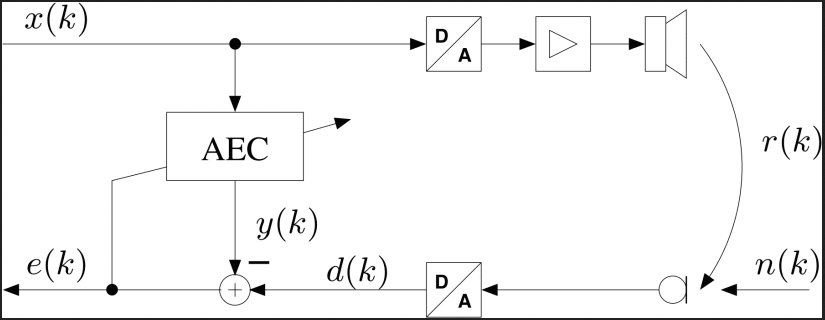
\includegraphics[width=\textwidth]{AEC_Block_Diagram}
		\caption{Block Diagram of an Acoustic Echo Cancellation System}
	\end{figure}
\end{frame}

\section{Theory}

\subsection{Algorithms}
\begin{frame}{Adaptive Algorithms}
The algorithms that we will be discussing today for Acoustic Echo Cancellation are:
	\begin{enumerate}
		\item Least Means Square (LMS)
		\item Frequency Domain Adaptive Filtering (FDAF)
	\end{enumerate}
\end{frame}

\begin{frame}{LMS Algorithm}
\textbf{Given:}
\begin{itemize}
	\item The (correlated) input signal samples ${u(1),u(2),u(3),...}$,
generated randomly
	\item The desired signal samples ${d(1),d(2),d(3),...}$ correlated
with ${u(1),u(2),u(3),...}$
\end{itemize}

	\begin{enumerate}
		\item Initialize the algorithm with an arbitrary parameter vector $w(0)$, for example $w(0) = 0$.
		\item Iterate for $n = 0,1,2,3,...,n_{max}$
			\begin{enumerate}[I]
				\item Read /generate a new data pair,\hfill $(u(n),d(n))$
				\item (Filter output) \hfill $y(n) = w(n)^T u(n) = \sum_{i=0}^{M-1} w_i(n)u(n-i)$
				\item (Output error) \hfill $e(n) = d(n) − y(n)$
				\item (Parameter adaptation) \hfill $w(n + 1) = w(n) + \mu u(n)e(n)$
			\end{enumerate}
	\end{enumerate}
\end{frame}

\begin{frame}{FDAF Algorithm}
For each block of M data samples do the following:\\
\begin{enumerate}
	\item  Compute the output of the filter for the block $kM,...,kM + M − 1$
	$\begin{bmatrix}
	\ubar{C}\\ 
	\ubar{y}
	\end{bmatrix} = IFFT\bigg(FFT(\begin{bmatrix}
	\ubar{w(k)}\\ 
	\ubar{0}
	\end{bmatrix})* FFT([\ubar{u}])\bigg)$
	\item Compute the correlation vector
	$\begin{bmatrix}
	\ubar{\phi}\\ \ubar{D}
	\end{bmatrix} = IFFT\bigg( FFT(\begin{bmatrix}
	\ubar{0}\\ 
	\ubar{e}
	\end{bmatrix})*\overline{FFT([\ubar{u}])} \bigg)$
	\item Update the parameters of the filter
	$FFT\begin{bmatrix}
	\ubar{w(k+1)}\\ 
	\ubar{0}
	\end{bmatrix} = FFT\begin{bmatrix}
	\ubar{w(k)}\\ 
	\ubar{0}
	\end{bmatrix} + \mu FFT\begin{bmatrix}
	\ubar{\phi}\\ 
	\ubar{0}
	\end{bmatrix}$
\end{enumerate}
\end{frame}


\begin{frame}{FDAF Block Diagram}
	\begin{figure}
		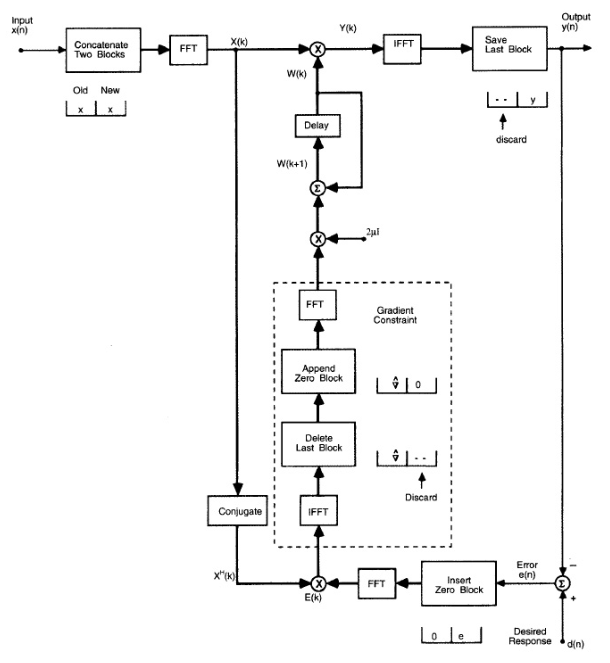
\includegraphics[width=\textwidth, height = 7.8cm]{FDAF_Block}
		\caption{Results with LMS algorithm, Step size = 0.05}
	\end{figure}
\end{frame}


\begin{frame}{Performance Parameters}
The performance parameter which is used here for the performance evaluation of different AEC Algorithms is known as \\ 
	\begin{center}
	\textbf{Echo Return Loss Enhancement (ERLE)}
	\end{center}

\textbf{What is ERLE?}\\
It is the measure of the amount (in dB) that the echo has been attenuated. It is mathematically defined as \\
	\begin{center}
	ERLE(dB) $= 10log_{10}{\frac{d^2(n)}{e^2(n)}}$
	\end{center}
Where,\\
$d(n)$ is the far-end echoed signal \\
$e(n)$ is the residual echo after cancellation
\end{frame}

\section{Results}
\begin{frame}{}
\begin{center}
\Huge Results
\end{center}
\end{frame}

\begin{frame}{LMS Algorithm}
	\begin{figure}
		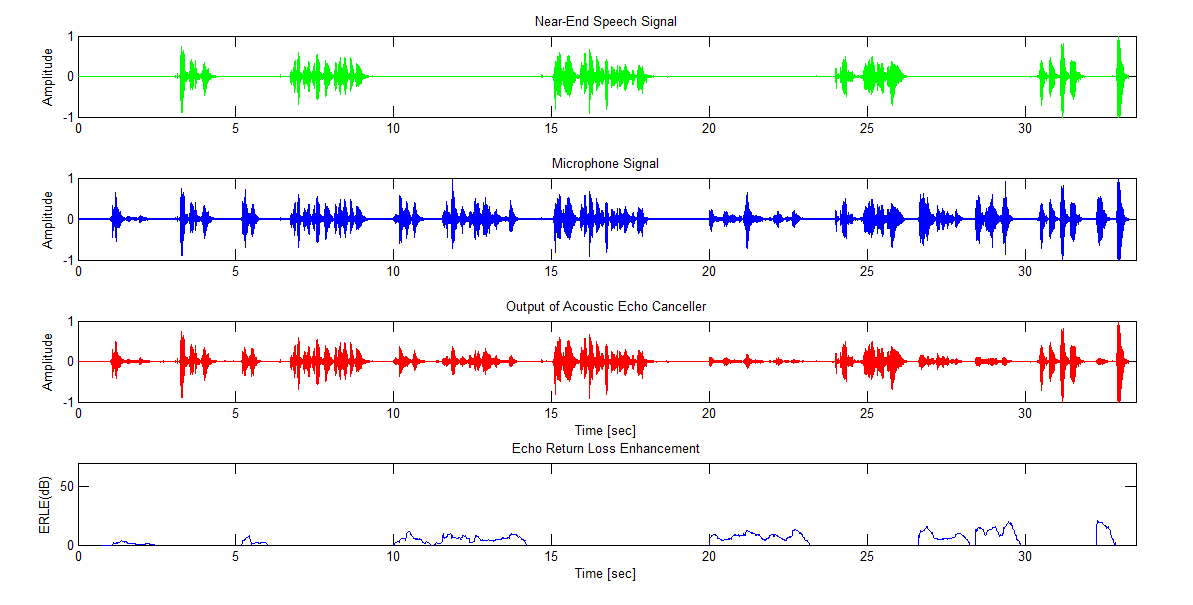
\includegraphics[width=\textwidth]{LMS_Result_5e-2}
		\caption{Results with LMS algorithm, Step size = 0.05}
	\end{figure}
\end{frame}

\begin{frame}{LMS Algorithm}
	\begin{figure}
		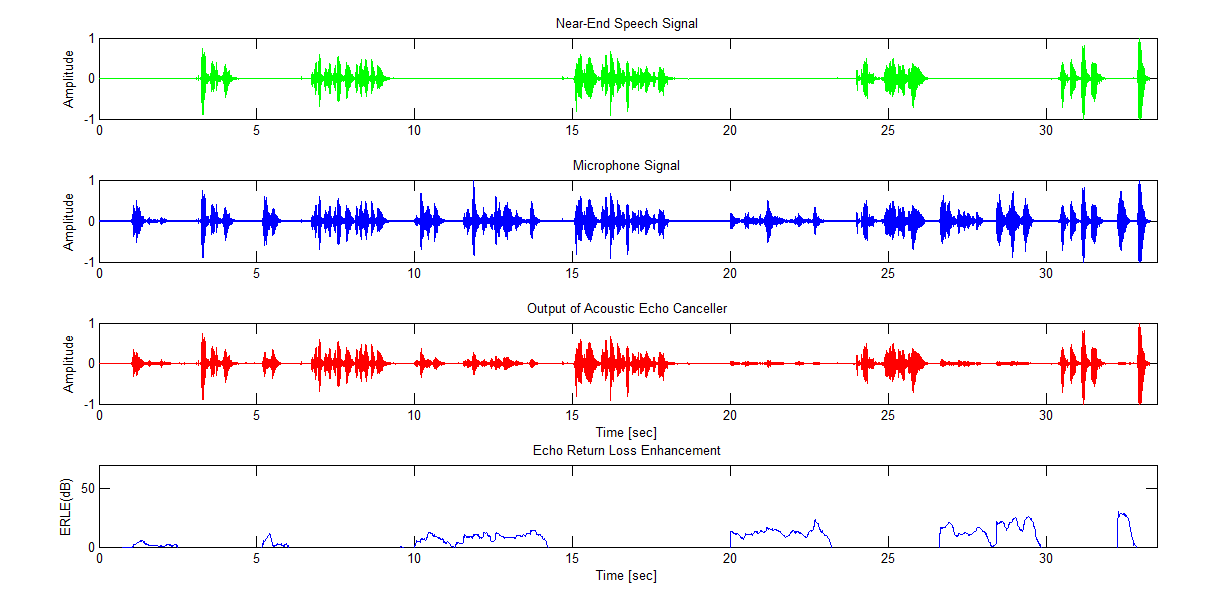
\includegraphics[width=\textwidth]{LMS_Result_13e-2}
		\caption{Results with LMS algorithm, Step size = 0.13}
	\end{figure}
\end{frame}


\begin{frame}{FDAF Algorithm}
	\begin{figure}
		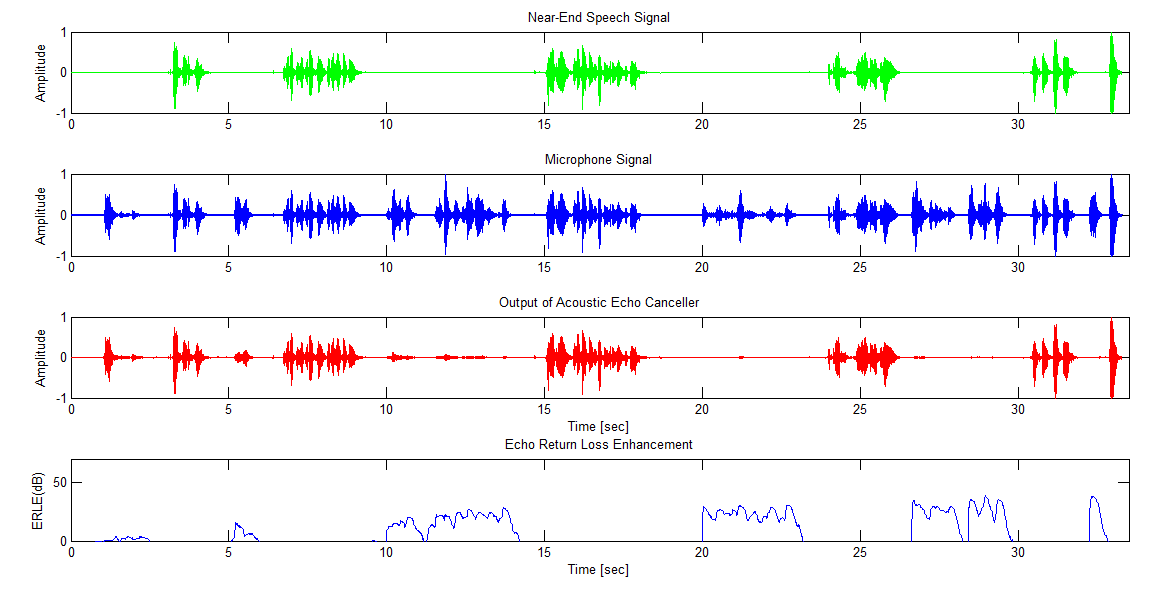
\includegraphics[width=\textwidth]{FDAF_Result}
		\caption{Results with FDAF algorithm, Step size = 0.025}
	\end{figure}
\end{frame}

\begin{frame}{FDAF Algorithm}
	\begin{figure}
		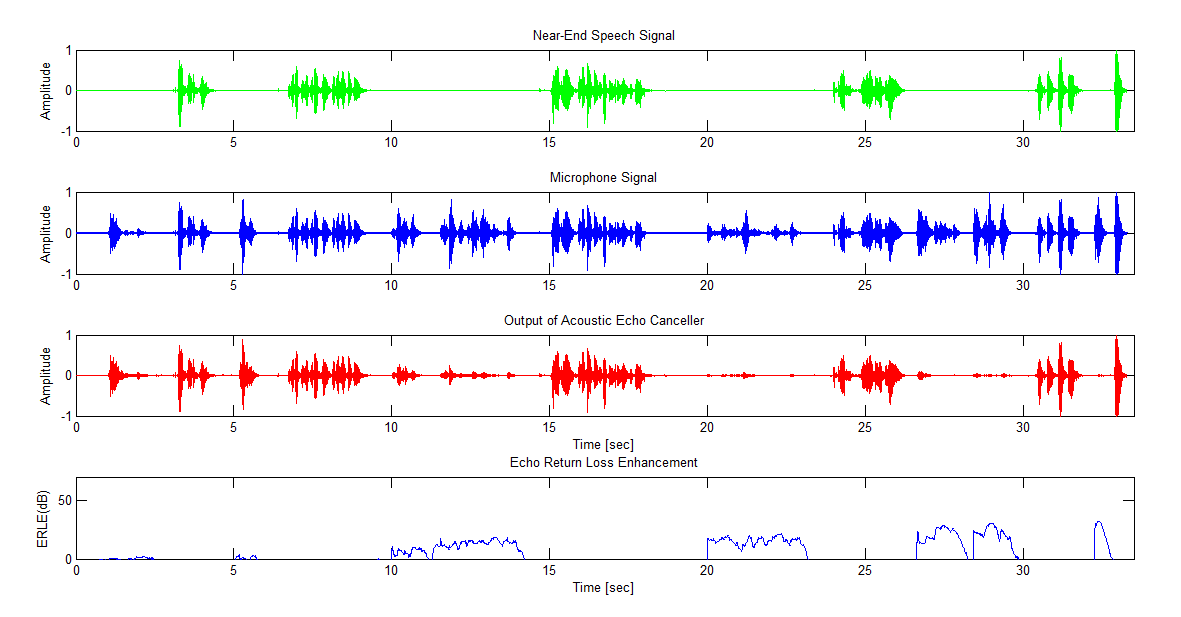
\includegraphics[width=\textwidth]{FDAF_Result_5e-2}
		\caption{Results with FDAF algorithm, Step size = 0.05}
	\end{figure}
\end{frame}

\nocite{*}
\section{Bibliography}
\begin{frame}{Bibliography}
	\bibliography{mybib}
	\bibliographystyle{ieeetr}
\end{frame}

\end{document}

